\documentclass[a4paper,12pt]{article}[abntex2]
\bibliographystyle{abntex2-alf}


% Definições de layout e formatação
\usepackage[a4paper, left=3.0cm, top=3.0cm, bottom=2.0cm, right=2.0cm]{geometry} % Personalização das margens do documento
\usepackage{setspace} % Controle do espaçamento entre linhas
\onehalfspacing % Espaçamento entre linhas de 1,5
\usepackage{indentfirst} % Indentação do primeiro parágrafo das seções
\usepackage{newtxtext} % Substitui a fonte padrão pela Times Roman
\usepackage{titlesec} % Personalização dos títulos de seções
\usepackage{ragged2e} % Melhor controle de justificação do texto
\usepackage[portuguese]{babel} % Adaptação para o português (nomes e hifenização)

% Pacotes de cabeçalho, rodapé e títulos
\usepackage{fancyhdr} % Customização de cabeçalhos e rodapés
\setlength{\headheight}{14.49998pt} % Altura do cabeçalho
\pagestyle{fancy}
\fancyhf{} % Limpa cabeçalho e rodapé
\rhead{\thepage} % Página no canto direito do cabeçalho

% Pacotes para tabelas
\usepackage{booktabs} % Melhora a qualidade das tabelas
\usepackage{tabularx} % Permite tabelas com larguras de colunas ajustáveis
\usepackage{float} % Melhor controle sobre o posicionamento de figuras e tabelas

% Pacotes para gráficos e imagens
\usepackage{graphicx} % Suporte para inclusão de imagens

\usepackage[utf8]{inputenc}
\usepackage{listingsutf8}

\lstset{
    language=R,                      
    basicstyle=\ttfamily\scalefont{1.0},
    keywordstyle=\color{blue},       
    stringstyle=\color{red},         
    commentstyle=\color{green},      
    numbers=left,                    
    numberstyle=\tiny\color{gray},   
    stepnumber=1,                    
    numbersep=5pt,                   
    backgroundcolor=\color{lightgray!10}, 
    frame=single,                    
    breaklines=true,                 
    captionpos=b,                    
    keepspaces=true,                 
    showspaces=false,                
    showstringspaces=false,          
    showtabs=false,                  
    tabsize=2,
     literate={á}{{\'a}}1
             {é}{{\'e}}1
             {í}{{\'i}}1
             {ó}{{\'o}}1
             {ú}{{\'u}}1
             {Ú}{{\'U}}1
             {â}{{\^a}}1
             {ê}{{\^e}}1
             {î}{{\^i}}1
             {ô}{{\^o}}1
             {û}{{\^u}}1
             {ã}{{\~a}}1
             {õ}{{\~o}}1
             {ç}{{\c{c}}}1,
}


% Pacotes para unidades e formatação numérica
\usepackage{siunitx} % Tipografia de unidades do Sistema Internacional e formatação de números
\sisetup{
  output-decimal-marker = {,},
  inter-unit-product = \ensuremath{{}\cdot{}},
  per-mode = symbol
}
\DeclareSIUnit{\real}{R\$}
\newcommand{\real}[1]{R\$#1}

% Pacotes para hiperlinks e referências
\usepackage{hyperref} % Suporte a hiperlinks
\usepackage{footnotehyper} % Notas de rodapé clicáveis em combinação com hyperref
\hypersetup{
    colorlinks=true,
    linkcolor=black,
    filecolor=magenta,      
    urlcolor=cyan,
    citecolor=black,        
    pdfborder={0 0 0},
}
\makeatletter
\def\@pdfborder{0 0 0} % Remove a borda dos links
\def\@pdfborderstyle{/S/U/W 1} % Estilo da borda dos links
\makeatother

% Pacotes para texto e outros
\usepackage{lipsum} % Geração de texto dummy 'Lorem Ipsum'
\usepackage[normalem]{ulem} % Permite o uso de diferentes tipos de sublinhados sem alterar o \emph{}

\begin{document}

\begin{titlepage}
    \centering
    \vspace*{1cm}
    \Large\textbf{INSPER – INSTITUTO DE ENSINO E PESQUISA}\\
    \Large ECONOMIA\\
    \vspace{1.5cm}
    \Large\textbf{Atividade Prática Supervisionada}\\
    \textbf{Modelagem Preditiva}\\
    \vspace{1.5cm}
    Prof. Dr. Paulo Cilas Marques Filho \\
    Prof. Auxiliar Luiza Tuler Veloso \\
    \vfill
    \normalsize
    Hicham Munir Tayfour, \href{mailto:hichamt@al.insper.edu.br}{hichamt@al.insper.edu.br}\\
    João Alonso Casella, \href{mailto:joaoac3@al.insper.edu.br}{joaoac3@al.insper.edu.br}\\
    Philipe Libretti Dias, \href{mailto:philipeld@al.insper.edu.br}{philipeld@al.insper.edu.br}\\

    \vfill
    São Paulo\\
    Outubro/2024
\end{titlepage}

\newpage
\tableofcontents
\thispagestyle{empty} % Esse comando remove a numeração de pagina da tabela de conteúdo

\newpage 
\listoffigures
\thispagestyle{empty} % Esse comando remove a numeração de pagina da tabela de figura

\newpage
\setcounter{page}{1} % Inicia a contagem de páginas a partir desta página
\justify
\onehalfspacing

\section*{\textbf{Parte Tórica}}
\addcontentsline{toc}{section}{Parte Tórica}

\subsection*{Questão 1: Árvores de Regressão}
\addcontentsline{toc}{subsection}{Questão 1: Árvores de Regressão}

As árvores de regressão são um método preditivo que se utiliza do algoritmo CART \textit{(Classification and Regression Trees)}, criado por Leo Braiman, Jerome Friedman, Richard Olsen e Charles Stone, em seu livro \textit{Classification and Regression Trees}, publicado em 1984. Nele, os autores formulam, portanto, tal algoritmo, inicialmente para a utilização no método de árvores de classificação, que possui o mesmo formato e aplicação da de regressão, porém com o objetivo de gerar categorias discretas, enquanto a outra busca gerar categorias numéricas.

O objetivo do algoritmo é, a partir de um conjunto de dados de treinamento, ser capaz de separá-los em diferentes categorias para que, dado que tal separação foi realizada com sucesso, ser capaz de, utilizando um outro conjunto de dados de teste, conseguir prever corretamente qual o destino de cada uma das novas informações, com o menor erro possível. A partir de um exemplo semelhante ao mostrado em sala de aula, a Figura \ref{fig1 - 1} assume a existência de dados de um banco, com os rótulos de \(Sim\) e \(Não\) referentes a se o cliente utilizou ou não o limite do cheque especial em mais de dois meses do ano. O ponto \(A\) determina o nó da raíz, onde a divisão entre os grupos, e os pontos onde há a escolha entre \(Sim\) e \(Não\)  são as folhas (ou terminais) da árvore.

\begin{figure}[H]
    \centering
    \caption{Exemplo de Árvore de Classificação} 
    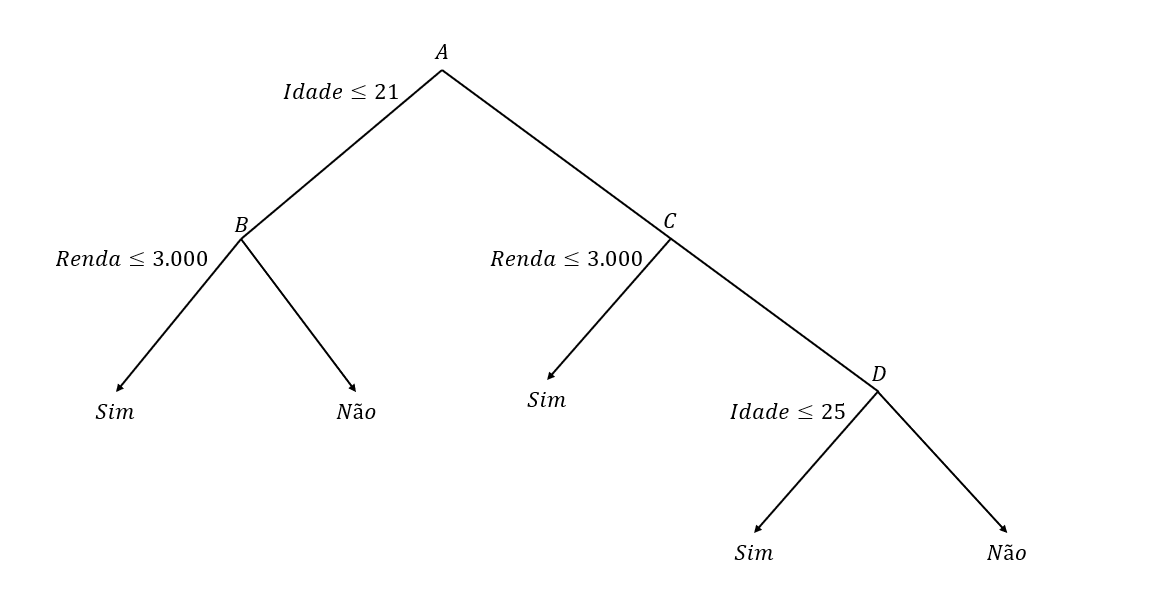
\includegraphics[width=1.0\textwidth]{APS/fig1 - 1.png}
    \label{fig1 - 1}
    
    \footnotesize{Fonte: Elaborado pelos autores.}
\end{figure}

A quantidade de nós e, por consequência, de divisões (ou \textit{splits}), na árvore de classificação é definida a partir da minimização do erro de classificação. O funcionamento da árvore de regressão é semelhante, porém, ao invés do erro de classificação, é utilizada a perda quadrática. Em termos gerais, dado \(y_i\) um dos dados de treinamento dentro de uma região \(R\), a equação da perda quadrática é dada por
\begin{equation}
    (\hat{j}, \hat{t}) = arg \min_{(j,t)} \left(\sum_{\{i: x_i \epsilon R_1\}}(y_i - \hat{y}_{R_1})^2 + \sum_{\{i: x_i \epsilon R_2\}}(y_i - \hat{y}_{R_2})^2 \right)
\end{equation}
com \(\hat{y}_{R_1}\) e \(\hat{y}_{R_2}\) sendo as médias das respostas dos dados de treinamento pertencentes às regiões \(R_1\) e \(R_2\).

Depois de definir o número de nós, o CART define uma constante \(c_j\) a partir da média das respostas presentes em 
\begin{equation}
    c_j = \frac{1}{n_j}\sum^m_{\{i: x_i \epsilon R_j\}}y_i
\end{equation}
que, assim, é o valor preditivo para qualquer das respostas dos dados de treinamento que se encontrarem na região \(R_j\).

Para ilustrar a árvore de regressão, a Figura \ref{fig2 - 1} demonstra uma situação em que há dados de treinamento de valores do metro quadrado de imóveis em uma cidade (em milhares de reais), além de informações da distância dele em relação ao centro da cidade e o número de crimes próximos ao imóvel no último mês, com as Regiões ótimas já definidas.

\begin{figure}[H]
    \centering
    \caption{Partição do espaço do exemplo de árvore de regressão} 
    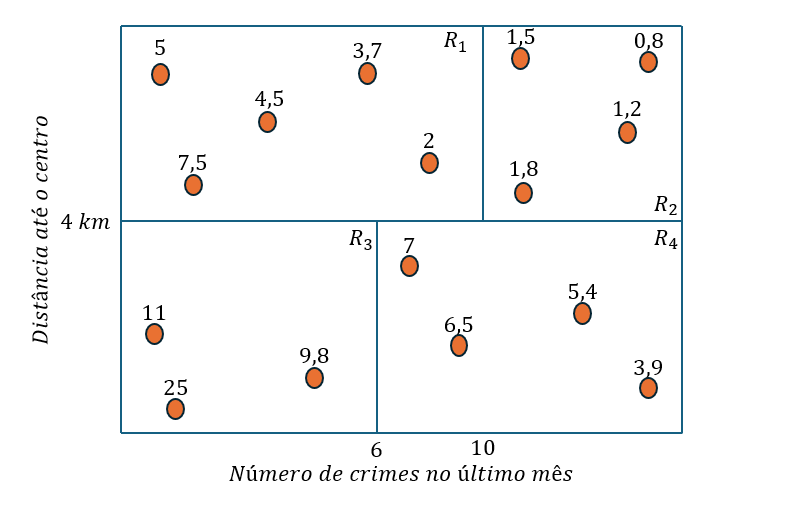
\includegraphics[width=1.0\textwidth]{APS/fig2 - 1.png}
    \label{fig2 - 1}
    
    \footnotesize{Fonte: Elaborado pelos autores.}
\end{figure}

A partir dessas informações, é possível, então, montar a Figura \ref{fig3 - 1}, que mostra a extensão da árvore de regressão do exemplo. Temos o nó \(A\) como o \textit{split} inicial, que separava as respostas entre imóveis que estavam menos ou exatamente a 4 quilômetros do centro da cidade e o resto. Então, o nó \(B\) separa, dentre aqueles iguais ou abaixo dos 4 km, quais dos imóveis tiveram um número de crimes próximos ao seu local no último mês igual ou abaixo de 6. Então, chegamos a duas folhas, representantes das regiões \(R_3\) e \(R_4\) na Figura \ref{fig2 - 1}, com as médias de suas observações sendo de 15,3 mil reais e 5,7 mil reais, respectivamente. Do outro lado, para imóveis a mais de 4 km de distância do centro da cidade, o nó \(C\) divide-os entre aqueles com número de crimes próximos no último mês igual ou menor que 10 e aqueles com valores maiores, assim chegando nas duas últimas folhas, representadas pelas regiões \(R_1\) e \(R_2\) na Figura \ref{fig2 - 1}. Enquanto a primeira possui uma média de 4,54 mil reais, a segunda possui uma menor entre seus valores, de somente 1,325 mil reais.

\begin{figure}[H]
    \centering
    \caption{Exemplo de Árvore de Regressão} 
    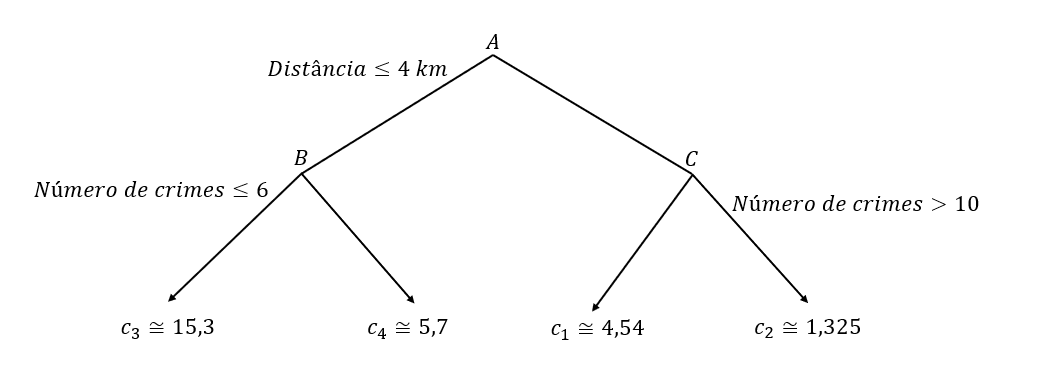
\includegraphics[width=1.0\textwidth]{APS/fig3 - 1.png}
    \label{fig3 - 1}
    
    \footnotesize{Fonte: Elaborado pelos autores.}
\end{figure}

\newpage
\subsection*{Questão 2: Bagging e Bootstrap}
\addcontentsline{toc}{subsection}{Questão 2: \textit{Bagging} e \textit{Bootstrap}}

Introduzindo a resposta objetivamente, o mecanismo de bagging é uma ferramenta de aprendizado de máquinas cujo objetivo principal é melhorar a precisão dos modelos preditivos; já o bootstrap é uma técnica estatística usada para gerar várias amostras aleatórias de um conjunto de dados, com reposição, a fim de estimar incertezas e obter uma visão mais precisa das estatísticas do modelo. No bagging, o bootstrap cria essas diferentes amostras para que múltiplos modelos sejam treinados de forma independente, permitindo que a combinação das previsões reduza a variância e aumente a estabilidade do modelo final.

Imagine que você quer prever o clima de amanhã e pede a opinião de várias pessoas, cada uma olhando para dados diferentes, mas todos tentando prever a mesma coisa. Cada pessoa pode ter uma resposta um pouco diferente, mas ao juntar as opiniões (por exemplo, pela média das respostas ou pela votação da maioria), você consegue uma previsão mais precisa e confiável. O bagging funciona de forma semelhante: ele cria várias versões de um modelo usando diferentes partes dos dados originais, como se fossem diferentes “opiniões” sobre o que o modelo deveria prever. Depois, ele junta essas “opiniões” (as previsões dos modelos) para dar um resultado final mais robusto e confiável. Assim, se algum modelo comete um erro, os outros modelos ajudam a corrigir, tornando a previsão mais estável e menos afetada por pequenos detalhes dos dados originais.

Para que isso funcione, o bagging usa uma técnica chamada bootstrap, que cria essas “partes diferentes” dos dados. O bootstrap, em termos simples, é um método que gera várias versões de um conjunto de dados a partir de uma única amostra. Ele faz isso pegando amostras aleatórias com reposição, o que significa que cada nova amostra pode ter repetição de alguns dados do conjunto original e deixar outros de fora. Dessa forma, o bootstrap cria amostras variadas, mas ainda representativas, permitindo que cada modelo no bagging treine em uma versão levemente diferente dos dados originais. Esse processo de criar novas amostras com o bootstrap permite que cada “opinião” do modelo seja um pouco diferente e, por isso, mais independente. Quando o bagging combina essas opiniões, ele produz uma previsão mais confiável e menos influenciada por erros individuais, como se estivesse juntando as melhores “perspectivas” sobre o clima para fazer uma única previsão mais sólida.

\begin{figure}[H]
    \centering
    \caption{Mecanismo de reamostragem do Bootstrap} 
    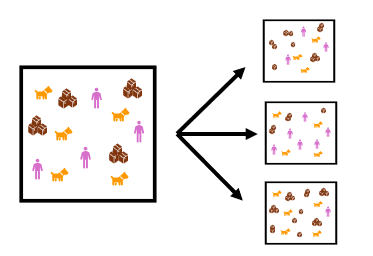
\includegraphics[width=0.5\textwidth]{APS/q2_fig1.png}
    \label{q2_fig1} 
    
    \footnotesize{Fonte: Elaborado pelos autores.}
\end{figure}


Para formalizar um pouco essa ideia, podemos olhar para as equações que representam o processo de bootstrap e bagging.
Dado um conjunto de dados \( D = \{x_1, x_2, \ldots, x_n\} \) com \( n \) observações, o bootstrap cria \( B \) amostras bootstrap \( D_1^{*}, D_2^{*}, \ldots, D_B^{*} \), onde cada amostra é obtida sorteando \( n \) vezes com reposição de \( D \). Isso quer dizer que cada nova amostra contém \( n \) observações que podem ser repetidas e também pode faltar algumas das observações originais.

Matematicamente, para cada amostra bootstrap \( D_i^{*} \):
\[
D_i^{*} = \{x_{i1}, x_{i2}, \ldots, x_{in}\}
\]
onde \( x_{ij} \) é escolhido aleatoriamente de \( D \) com reposição. No total, temos \( B \) amos tras.

Cada amostra bootstrap permite calcular estimativas independentes de algum parâmetro de interesse, digamos uma média ou variância. Por exemplo, para cada amostra \( D_i^{*} \), uma estatística \( \hat{\theta}_i^{*} \) é calculada:
\[
\hat{\theta}_i^{*} = \text{estatística}(D_i^{*})
\]
Ao calcular \( B \) estimativas \( \hat{\theta}_1^{*}, \hat{\theta}_2^{*}, \ldots, \hat{\theta}_B^{*} \), podemos combinar essas estimativas para obter uma média \( \hat{\theta}_{\text{bootstrap}} \):
\[
\hat{\theta}_{\text{bootstrap}} = \frac{1}{B} \sum_{i=1}^{B} \hat{\theta}_i^{*}
\]

Já o processo do bagging segue três etapas principais, começando pela criação das amostras, passando pelo treinamento, predições e, por fim, agrupamento.

\begin{figure}[H]
    \centering
    \caption{Estrutura de funcionamento Bagging} 
    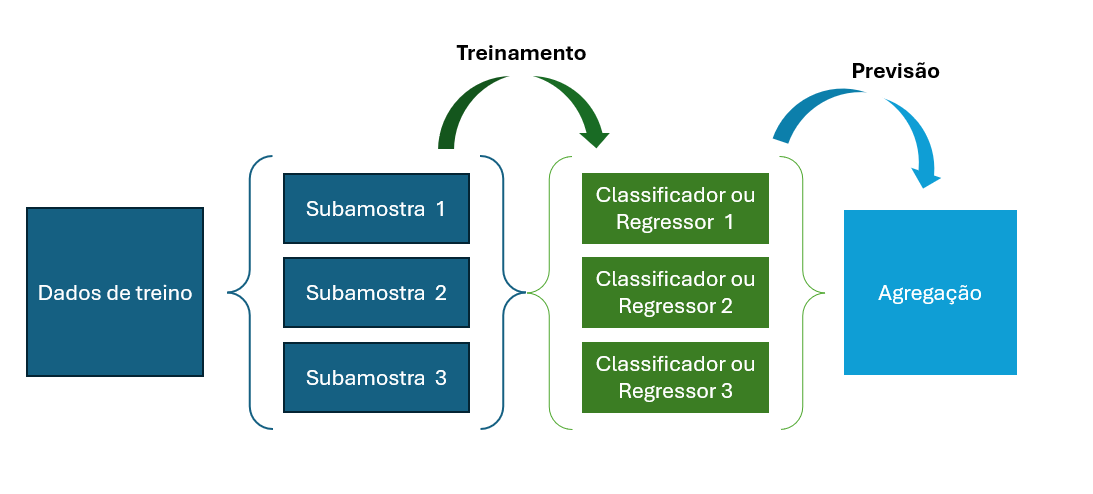
\includegraphics[width=1.0\textwidth]{APS/q2_fig2.png}
    \label{q2_fig2} 
    \footnotesize{Fonte: Elaborado pelos autores.}
\end{figure}

Como vimos, o bootstrap é usado para gerar amostras aleatórias \( D_1^{*}, D_2^{*}, \ldots, D_B^{*} \) a partir do conjunto de dados original, sempre com reposição. Isso significa que cada amostra bootstrap é única, mas ainda representativa do conjunto total, e pode conter repetições de alguns dados enquanto outros dados podem ficar de fora. 

Na segunda etapa, usamos essas amostras para treinar múltiplos modelos independentes. Para cada amostra \( D_i^{*} \), treinamos um modelo \( f_i \) específico. No final, teremos um conjunto de \( B \) modelos, denotados por \( f_1, f_2, \ldots, f_B \), onde cada um aprendeu a partir de uma amostra levemente diferente do conjunto de dados original. Esse treinamento independente entre os modelos é o que permite que o bagging aproveite o poder de combinações de previsões.

A última etapa é a combinação das previsões dos modelos, e essa etapa varia conforme o tipo de problema que estamos resolvendo. Para problemas de regressão, onde o objetivo é prever um valor contínuo, a previsão final para uma nova entrada \( x_{\text{new}} \) é dada pela média das previsões de todos os modelos. Em termos matemáticos, temos:
\[
\hat{y} = \frac{1}{B} \sum_{i=1}^{B} f_i(x_{\text{new}})
\]
Essa média suaviza as diferenças entre as previsões individuais, resultando em uma previsão final mais estável.

Para problemas de classificação, onde queremos categorizar uma entrada, a combinação das previsões usa a votação majoritária. Aqui, a previsão final é a categoria mais comum entre as previsões dos \( B \) modelos, expressa por:
\[
\hat{y} = \text{mode}\{f_1(x_{\text{new}}), f_2(x_{\text{new}}), \ldots, f_B(x_{\text{new}})\}
\]
Essa votação ajuda a reduzir o impacto de erros individuais, pois a categoria que a maioria dos modelos sugere é mais provável de ser a correta.

\newpage
\subsection*{Questão 3: Aleatorização de \textit{Splits} e \textit{Random Forests}}
\addcontentsline{toc}{subsection}{Questão 3: Aleatorização de \textit{Splits} e \textit{Random Forests}}

O mecanismo de aleatorização dos \textit{splits} criado por Breiman surge de um dos principais problemas observados em árvores de classificação: o viés. Ao criar uma árvore utilizando somente uma base de dados para treinamento, pode ocorrer um \textit{overfitting} do modelo aos dados iniciais, de forma que ele não tenha boa eficácia na previsão de futuros dados de teste. Dessa forma, foi proposto que o processo passasse por duas etapas de aleatorização, com o objetivo de reduzir tal viés.

O primeiro processo é chamado, como visto na questão anterior, de \textit{bootstrap}, que envolve, a partir dos dados de treinamento, criar outras bases aleatorizando os dados iniciais. Então, a partir das novas informações, é possível realizar árvores para cada iteração dos dados de treinamento. Porém, para criar tais árvores novas, será realizado um segundo processo de aleatorização, em que, para cada iteração, serão sorteados somente algumas regiões criadas pelos nós para criar a árvore. Esse processo é realizado a fim de frear o possível aumento da variância causado por realizar várias árvores utilizando todas as regiões da base de dados, assim sendo capaz de conter o \textit{trade-off} entre a redução do viés, porém com potenciais aumentos na variância causados pelo \textit{bootstrap}.

Por fim, a partir de um novo conjunto de dados, são realizadas as previsões com cada árvore e, a partir de um processo chamado de agregação, é determinada, por maioria, a previsão da \textit{Random Forest} criada. Para exemplificar o processo, tomemos a árvore da Figura ~\ref{fig1 - 1} como exemplo. Criando um gráfico que demonstra uma possível distribuição de dados de treinamento, a Figura ~\ref{fig3 - 1} (Nela, 1 refere-se a $Sim$ da outra figura e 0 a $Não$, para criar uma \textit{Random Forest}, o necessário seria, a partir das respostas de treinamento, criar outros \textit{datasets} aleatorizados, assim realizando o \textit{bootstrap} e, então, formar novas árvores com regiões também aleatórias e observar suas previsões com um dado de teste. Por fim, então realizado o processo de agregação, seria possível observar a previsão da \textit{Random Forest} completa sobre se os clientes do banco utilizaram o limite do cheque especial no último mês ou não.

\begin{figure}[H]
    \centering
    \caption{Exemplo de Distribuição de Dados da Árvore de Classificação} 
    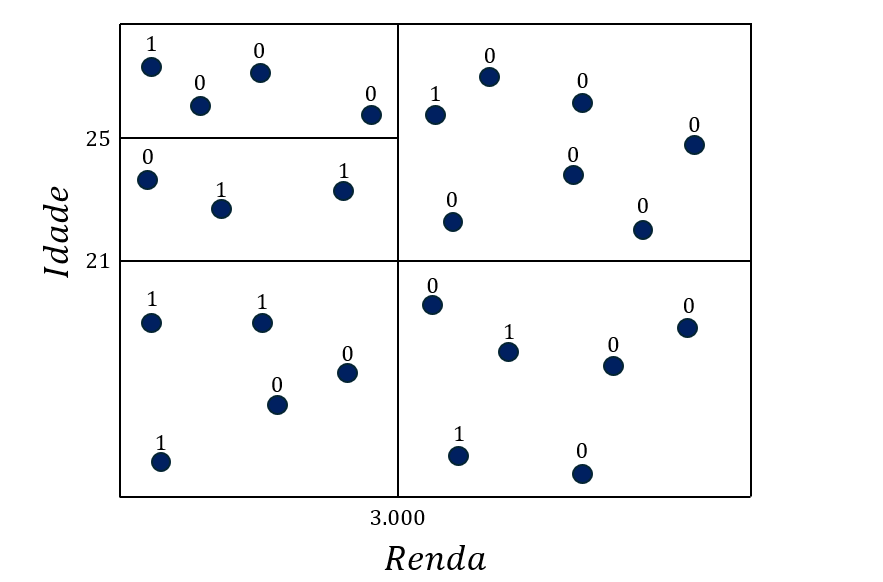
\includegraphics[width=1.0\textwidth]{APS/fig1 - 3.png}
    \label{fig1 - 3}
    
    \footnotesize{Fonte: Elaborado pelos autores.}
\end{figure}
\newpage
\subsection*{Questão 4: Erro Out-of-bag - Random Forest}
\addcontentsline{toc}{subsection}{Questão 4: Erro Out-of-bag - Random Forest}

O erro \textit{out-of-bag} (\textbf{OOB}) é uma forma de estimativa interna do erro de generalização de uma \textit{Random Forest}, no qual não se faz necessário um conjunto de dados específico para sua verificação. Tal estimativa usa da propriedade do \textit{Bootstrap}, a mesma usada para a construção da \textit{Random Forest}.

Na construção da \textit{Random Forest} , cada árvore é construída ou treinada usando uma amostra \textit{bootstrap} do conjunto de dados utilizado para realizar os treinamento. Tal processo uso da amostragem aleatória com dados que sofreram reposição, ou seja, a mesma observação pode ser vista mais de uma vez nos conjuntos de treinamento. Desse processo de reamostragem aleatória com reposição surge um resultado teórico indicando que cerca de 63,2\% das observações são selecionadas em cada amostra bootstrap, enquanto as observações não selecionadas, aproximadamente 36,8\%, são denominadas \textbf{OOB} para uma árvore em específico.

Assim chegamos que o cálculo do erro \textbf{OOB} vem do aproveitamento das observações não utilizadas no treino de cada árvore. Para cada observação no conjunto de treinamento, vemos quais árvores não a utilizaram em seu treinamento, essas são as árvores \textbf{OOB} para essa observação. Em seguida,.  utiliza-se essas árvores para prever o valor ou a classe da observação. No caso de classificação, realiza-se uma votação majoritária entre as predições das árvores OOB; na regressão, calcula-se a média das predições.

Na classificação, registra-se se a predição está correta ou não; na regressão, calcula-se a diferença entre o valor predito e o valor real, usando o erro absoluto ou quadrático. Repetindo esse processo para todas as observações, chegamos na taxa de erro total, que é o número de predições incorretas dividido pelo total de observações, ou o erro médio no caso de regressão.

Para exemplificar, considere um cenário com um conjunto de dados contendo 10 observações e uma \textit{Random Forest} com 5 árvores. Durante o treino das árvores, cada uma seleciona uma amostra \textit{bootstrap} diferente do conjunto de dados, resultando em diferentes conjuntos de observações OOB para cada árvore. Por exemplo: \begin{itemize}
    \item \textbf{Árvore 1}: amostra \textit{bootstrap} [1, 2, 2, 3, 4, 5, 5]; observações \textbf{OOB} [6, 7, 8, 9, 10].
    \item \textbf{Árvore 2}: amostra \textit{bootstrap} [2, 3, 3, 4, 5, 6, 7]; observações \textbf{OOB} [1, 8, 9, 10].
    \item \textbf{Árvore 3}: amostra \textit{bootstrap} [1, 3, 5, 7, 9]; observações \textbf{OOB} [2, 4, 6, 8, 10].
    \item \textbf{Árvore 4}: amostra \textit{bootstrap} [2, 4, 6, 8, 10]; observações \textbf{OOB} [1, 3, 5, 7, 9].
    \item \textbf{Árvore 5}: amostra \textit{bootstrap} [1, 2, 3, 6, 7]; observações \textbf{OOB} [4, 5, 8, 9, 10].
\end{itemize}

Para cada observação, vemos árvores que não a utilizaram no treinamento e se realiza as previsões. Por exemplo, para a observação 1, as árvores \textbf{OOB} são a 2 e a 4. Supondo que ambas prevejam a classe "A" e que a classe real também seja "A", a previsão é considerada correta. Para a observação 6, as árvores \textbf{OOB} são a 1 e a 3. Se a previsão da Árvore 1 for "A" e da Árvore 3 for "B", e a classe real for "A", pode haver um empate na votação, necessitando de um critério adicional para desempate.

Após fazer as previsões para todas as observações, calcula-se o erro \textbf{OOB} total. Supondo que, das 10 observações, 2 foram preditas incorretamente, o erro \textbf{OOB} será de 20\%, calculado como \( \frac{2}{10} \).

O erro \textbf{OOB} apresenta várias vantagens. Ele economiza dados, já que não é necessário separar um conjunto de validação, é computacionalmente eficiente e reduz o tempo de processamento. Além disso, fornece uma estimativa imparcial do erro de generalização, já que cada observação é predita utilizando apenas as árvores que não a viram durante o treinamento.

Entretanto, é importante considerar que, em conjuntos de dados muito pequenos ou com um número reduzido de árvores, a estimativa do erro \textbf{OOB} pode ser menos precisa.

Sendo assim, o erro \textit{out-of-bag} é uma ferramenta poderosa para avaliar o desempenho de uma \textit{Random Forest} sem a necessidade de dados adicionais para validação. Ao aproveitar a estrutura inerente do algoritmo, ele fornece uma estimativa eficiente e imparcial do erro de generalização do modelo, contribuindo para a eficácia e a praticidade do uso de \textit{Random Forests} em diversos problemas de previsão.


\newpage
\section*{\textbf{Aplicação 1 : Um Problema de Churn}}
\addcontentsline{toc}{section}{Aplicação 1 : Um Problema de Churn}

Neste estudo, aplicamos quatro modelos de classificação (Regressão Logística, Árvore de Decisão, Random Forest e CatBoost) para prever o churn de clientes de uma instituição bancária, utilizando um conjunto de dados que inclui diversas variáveis explicativas. Nosso objetivo principal é identificar qual modelo apresenta o melhor desempenho para a previsão do churn, focando nas métricas de AUC, ponto de corte (Best\_Threshold), especificidade e sensibilidade. 

A Tabela \ref{fig:i2A1} mostra uma comparação quantitativa das métricas ROC de cada modelo, enquanto a Figura \ref{fig:i1A1} ilustra as curvas ROC para uma análise visual do desempenho de cada método.

\begin{itemize}
    \item \textbf{CatBoost}: Este modelo apresentou a maior Área sob a Curva (AUC = 0.8622), indicando um excelente poder preditivo para distinguir entre clientes que cancelaram ou não os serviços. O ponto de corte ideal para o CatBoost foi de 0.1886, o que maximiza o equilíbrio entre sensibilidade (76.62\%) e especificidade (80.17\%). Esse modelo se destacou por apresentar tanto alta sensibilidade quanto alta especificidade, sugerindo ser adequado para situações onde é importante minimizar tanto falsos negativos quanto falsos positivos.

    \item \textbf{Random Forest}: Com uma AUC de 0.8549, o Random Forest foi o segundo melhor modelo em termos de desempenho. O ponto de corte ótimo para este modelo foi 0.2243, com uma sensibilidade de 75.48\% e uma especificidade de 79.95\%. Embora a especificidade seja ligeiramente menor que a do CatBoost, o Random Forest ainda mantém um bom equilíbrio entre as duas métricas, tornando-o uma opção robusta para previsão de churn. 

    \item \textbf{Regressão Logística}: A Regressão Logística apresentou uma AUC de 0.7657, que é inferior aos modelos baseados em árvores, indicando menor poder preditivo. O ponto de corte ótimo foi 0.2054, resultando em uma especificidade de 71.09\% e sensibilidade de 69.38\%. Este modelo é mais simples e interpretável, o que pode ser uma vantagem em cenários onde a interpretabilidade é mais valorizada que o desempenho puro, mas tem uma precisão preditiva inferior quando comparado ao CatBoost e ao Random Forest.

    \item \textbf{Árvore de Decisão}: Este modelo apresentou o menor AUC entre os quatro (0.7533), indicando um desempenho mais modesto. Com um ponto de corte de 0.1966, a especificidade foi de 81.54\%, enquanto a sensibilidade ficou em 62.5\%. Apesar de ter uma especificidade relativamente alta, a baixa sensibilidade sugere que ele pode não ser a melhor escolha para um cenário onde a identificação correta dos clientes que irão cancelar (minimizar falsos negativos) é crucial.
\end{itemize}

\begin{figure}[H]
    \centering
    \caption{Curvas R.O.C dos Modelos para previsão de Churn} 
    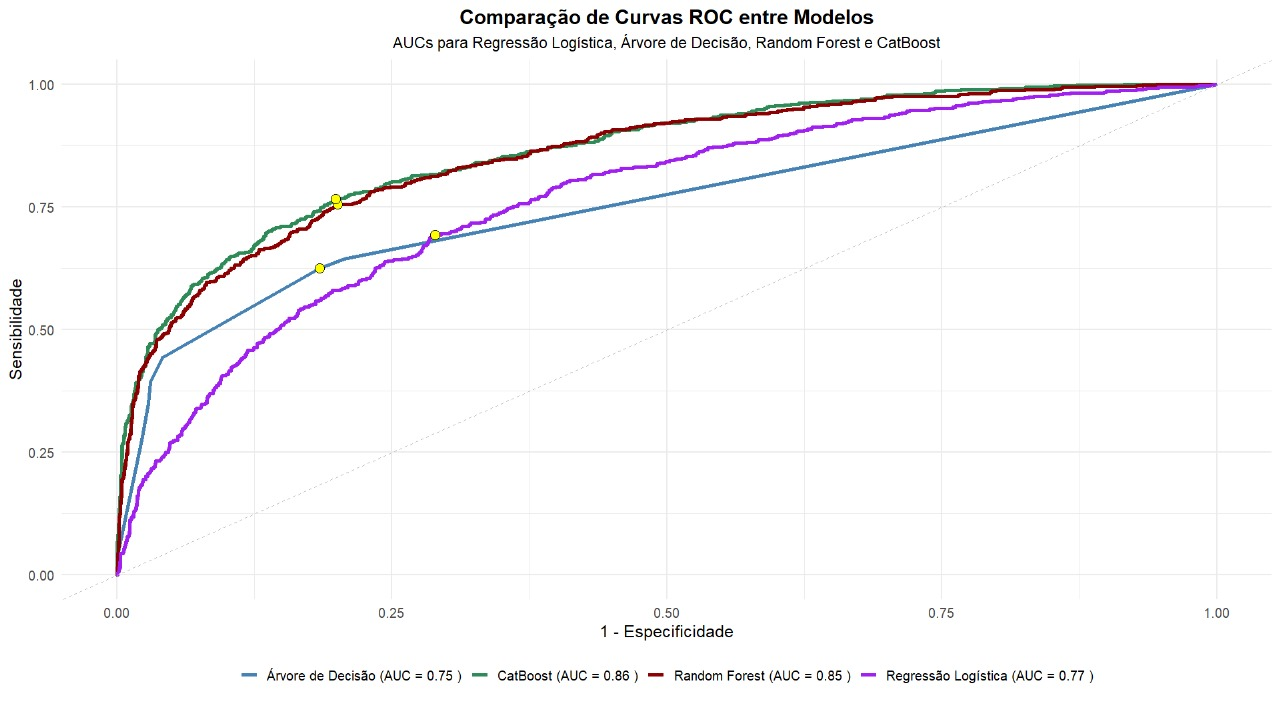
\includegraphics[width=1.0\textwidth]{APS/i1A1.png}
    \label{fig:i1A1}
    
    \footnotesize{Fonte: Dados de Churn; Elaborado pelos autores.}
\end{figure}

\begin{figure}[H]
    \centering
    \caption{Tabela de Comparação dos Modelos para previsão de Churn} 
    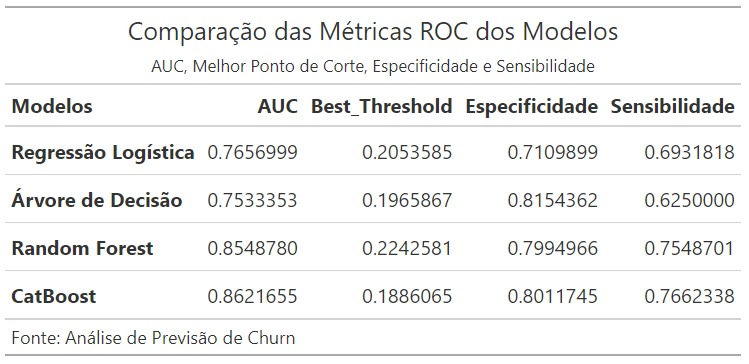
\includegraphics[width=1.0\textwidth]{APS/i2A1.png}
    \label{fig:i2A1}
    
    \footnotesize{Fonte: Dados de Churn; Elaborado pelos autores.}
\end{figure}

\subsection*{\textbf{Discussão dos Resultados de Classificação}}
\addcontentsline{toc}{subsection}{Discussão dos Resultados de Classificação}


Ao observarmos a Tabela \ref{fig:i2A1} e a Figura \ref{fig:i1A1}, é evidente que os modelos CatBoost e Random Forest apresentam desempenhos superiores em termos de AUC, o que reflete uma maior capacidade de discriminação entre as classes de churn e não churn. No entanto, a escolha final do modelo depende de outros fatores específicos ao contexto de aplicação:

\begin{itemize}
    \item Se o objetivo é reduzir ao máximo os falsos negativos, ou seja, identificar corretamente os clientes que provavelmente irão cancelar, o CatBoost pode ser a melhor escolha devido à sua alta sensibilidade combinada com uma especificidade igualmente forte.
    \item Em casos onde a interpretabilidade é crucial, a Regressão Logística, apesar de seu menor desempenho, pode ser preferível por sua simplicidade e facilidade de interpretação.
    \item A Árvore de Decisão, embora tenha especificidade alta, possui sensibilidade baixa, indicando uma limitação em identificar corretamente todos os clientes que irão churn. Assim, esse modelo poderia ser menos ideal para a tarefa de previsão de churn em casos onde identificar potenciais cancelamentos é prioritário.
\end{itemize}

Os resultados sugerem que, para este conjunto de dados e com os modelos avaliados, o CatBoost e o Random Forest são as melhores escolhas em termos de performance geral, proporcionando um bom equilíbrio entre sensibilidade e especificidade. A escolha entre os dois pode depender da necessidade de interpretabilidade versus ligeiras melhorias no desempenho preditivo.




\newpage
\section*{\textbf{Aplicação 2: Preço de automóveis usados}}
\addcontentsline{toc}{section}{Aplicação 2: Preço de automóveis usados}

Neste estudo, realizamos uma análise preditiva de preços de veículos usados da marca Mercedes utilizando quatro métodos de regressão: Regressão Linear Múltipla, Árvore de Regressão, Random Forest e CatBoost. O objetivo é prever a variável \textbf{price} a partir de outras características dos veículos. A Tabela \ref{fig:i2A2} apresenta uma comparação das métricas EQM (Erro Quadrático Médio) de treino e teste, bem como o RMSE (Raiz do Erro Quadrático Médio) no conjunto de teste para cada modelo.

\begin{itemize}
    \item \textbf{Regressão Linear Múltipla}: Este modelo apresentou um EQM de teste de 45.4987 e RMSE de 6.7453, indicando que há uma diferença significativa entre o erro médio quadrático no conjunto de treino (46.0301) e no teste. Esse modelo, sendo o mais simples, pode não capturar completamente as complexidades dos dados, resultando em uma performance inferior quando comparado a modelos mais complexos como Random Forest e CatBoost.

    \item \textbf{Árvore de Regressão}: A Árvore de Regressão apresentou desempenho semelhante à Regressão Linear, com um EQM de teste de 45.5772 e um RMSE de 6.7511. Esse modelo é capaz de capturar algumas não-linearidades nos dados, mas ainda assim apresenta um erro considerável, indicando que o modelo talvez seja insuficiente para capturar todas as nuances dos preços de veículos usados.

    \item \textbf{Random Forest}: Com um EQM de teste significativamente menor (17.8729) e RMSE de 4.2276, o Random Forest se destacou em relação aos modelos anteriores. Isso sugere que o modelo foi capaz de capturar bem as variações nos preços, provavelmente devido à capacidade de combinar múltiplas árvores de decisão, o que melhora a robustez e precisão das previsões.

    \item \textbf{CatBoost}: Este modelo apresentou o menor erro entre todos, com um EQM de teste de 17.2699 e RMSE de 4.1557. Esse resultado indica que o CatBoost é o modelo com melhor desempenho, sendo capaz de aprender as complexidades do conjunto de dados e fornecer previsões de preços de veículos mais precisas. O CatBoost, por ser um modelo de boosting, tende a melhorar continuamente as previsões ao corrigir erros em iterações sucessivas, o que pode explicar sua alta precisão neste caso.
\end{itemize}

\begin{figure}[H]
    \centering
    \caption{Tabela de Comparação dos Modelos para Previsão de Preços de Carros Usados} 
    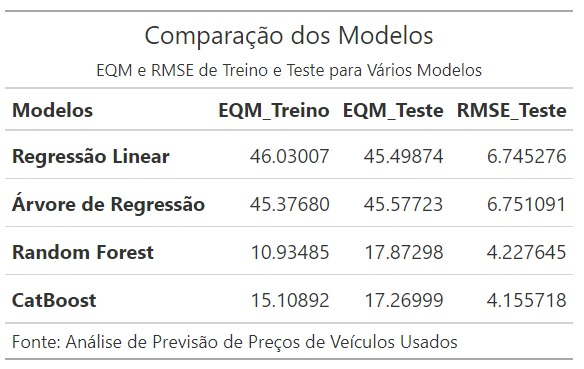
\includegraphics[width=1.0\textwidth]{APS/i1A2.png}
    \label{fig:i2A2}
    
    \footnotesize{Fonte: Dados de Preços carros Usados; Elaborado pelos autores.}
\end{figure}

\subsection*{\textbf{Discussão dos Resultados de Regressão}}
\addcontentsline{toc}{subsection}{Discussão dos Resultados de Regressão}


A Tabela \ref{fig:i2A2} revela que, entre os modelos analisados, o CatBoost e o Random Forest apresentaram os melhores desempenhos, com RMSE significativamente menores em comparação à Regressão Linear Múltipla e à Árvore de Regressão. Esse comportamento é esperado, pois tanto o Random Forest quanto o CatBoost são modelos baseados em árvores e são capazes de lidar melhor com a complexidade e a variabilidade dos dados.

\begin{itemize}
    \item \textbf{Interpretação dos Erros}: A diferença entre os RMSEs de teste sugere que a Regressão Linear e a Árvore de Regressão podem não ser capazes de capturar as interações complexas entre as variáveis. O erro mais alto nos modelos lineares indica uma possível subestimativa dos valores de preço.
    \item \textbf{Robustez dos Modelos de Ensemble}: Tanto o Random Forest quanto o CatBoost são robustos em relação ao overfitting, especialmente o CatBoost, que utiliza técnicas de boosting para corrigir erros iterativamente. Esse processo permite que o CatBoost apresente um desempenho ligeiramente superior, capturando melhor as nuances dos dados e fornecendo previsões mais precisas.
    \item \textbf{Considerações sobre Interpretabilidade e Complexidade}: A Regressão Linear e a Árvore de Regressão, embora menos precisas, são mais interpretáveis, o que pode ser útil em cenários onde a transparência do modelo é prioritária. No entanto, para maximizar a precisão da previsão, o CatBoost se mostrou a melhor escolha.
\end{itemize}

Dessa forma, os resultados sugerem que, para o problema de previsão de preços de veículos usados, o \textbf{CatBoost} e o \textbf{Random Forest} são as opções mais recomendadas, sendo que o CatBoost apresentou um leve benefício adicional em termos de erro de previsão. Esses modelos, ao capturar interações complexas nos dados, fornecem maior precisão, o que é fundamental para aplicações onde uma estimativa precisa de preços é essencial.


\end{document}